% !TeX root = ../../Skript.tex
\cohead{\Large\textbf{Satz vom Nullprodukt/Produktform}}
\fakesubsection{Satz vom Nullprodukt/Produktform}
\setlength{\qrheight}{2.5cm}%
\newlength{\produktbox}
\iftoggle{qrcode}{\setlength{\produktbox}{\textwidth-\qrheight}}{\setlength{\produktbox}{\textwidth}}%
\adjustbox{valign=t}{\begin{minipage}{\produktbox}
    Die Produktform ist nach der Scheitelform und der Hauptform die dritte und letzte Darstellungsform für quadratische Funktionen. Um den Aufbau der Produktform nachvollziehen zu können, muss man den Satz vom Nullprodukt (SvN) kennen.

    Das Produkt zweier Zahlen \(a\) und \(b\) ist genau dann Null, wenn entweder \(a\) Null ist oder \(b\) Null ist:
\end{minipage}}%
\iftoggle{qrcode}{%
    \adjustbox{valign=t, min height=\qrheight, max height = \qrheight}{\href{https://www.geogebra.org/m/weczkmhe}{
\includegraphics[width=\qrheight]{\quadFkt/pics/ProduktformQR.png}}}%
}{}%
\begin{tcolorbox}\centering
	\(\textcolor{loestc}{a\cdot b=0\ \Leftrightarrow\ a=0\text{ oder }b=0}\)
\end{tcolorbox}
Liegt die Funktionsgleichung einer quadratischen Funktion in der folgenden Form vor, so spricht man von der Produktform:
\[f(x)=\textcolor{loes}{a\cdot \left(x-x_1\right)\left(x-x_2\right), \quad a\neq 0}\]
\begin{itemize}
	\item Streckfaktor \(a\): \textcolor{loes}{Streckt die Parabel in y-Richtung.}\vspace{0.8cm}
	\item \(x_1,\ x_2\): \textcolor{loes}{Nullstellen der Parabel. Setzt man für \(x\) den Wert \(x_1\) oder \(x_2\) ein, so nimmt jeweils eine der beiden Klammern den Wert 0 an. Gemäß SvN wird dann der gesamte Funktionswert Null.}\vspace{0.8cm}
\end{itemize}
\begin{tcolorbox}\centering
	\textcolor{loestc}{ACHTUNG: Die Produktform kann nur dann aufgestellt werden, wenn die quadratsche Funktion mindestens eine (doppelte) Nullstelle hat.}
\end{tcolorbox}

\begin{minipage}{\textwidth}
		\adjustbox{valign=t, padding=0ex 0ex 3ex 0ex}{\begin{minipage}{\textwidth/\real{3}-2ex}\centering
			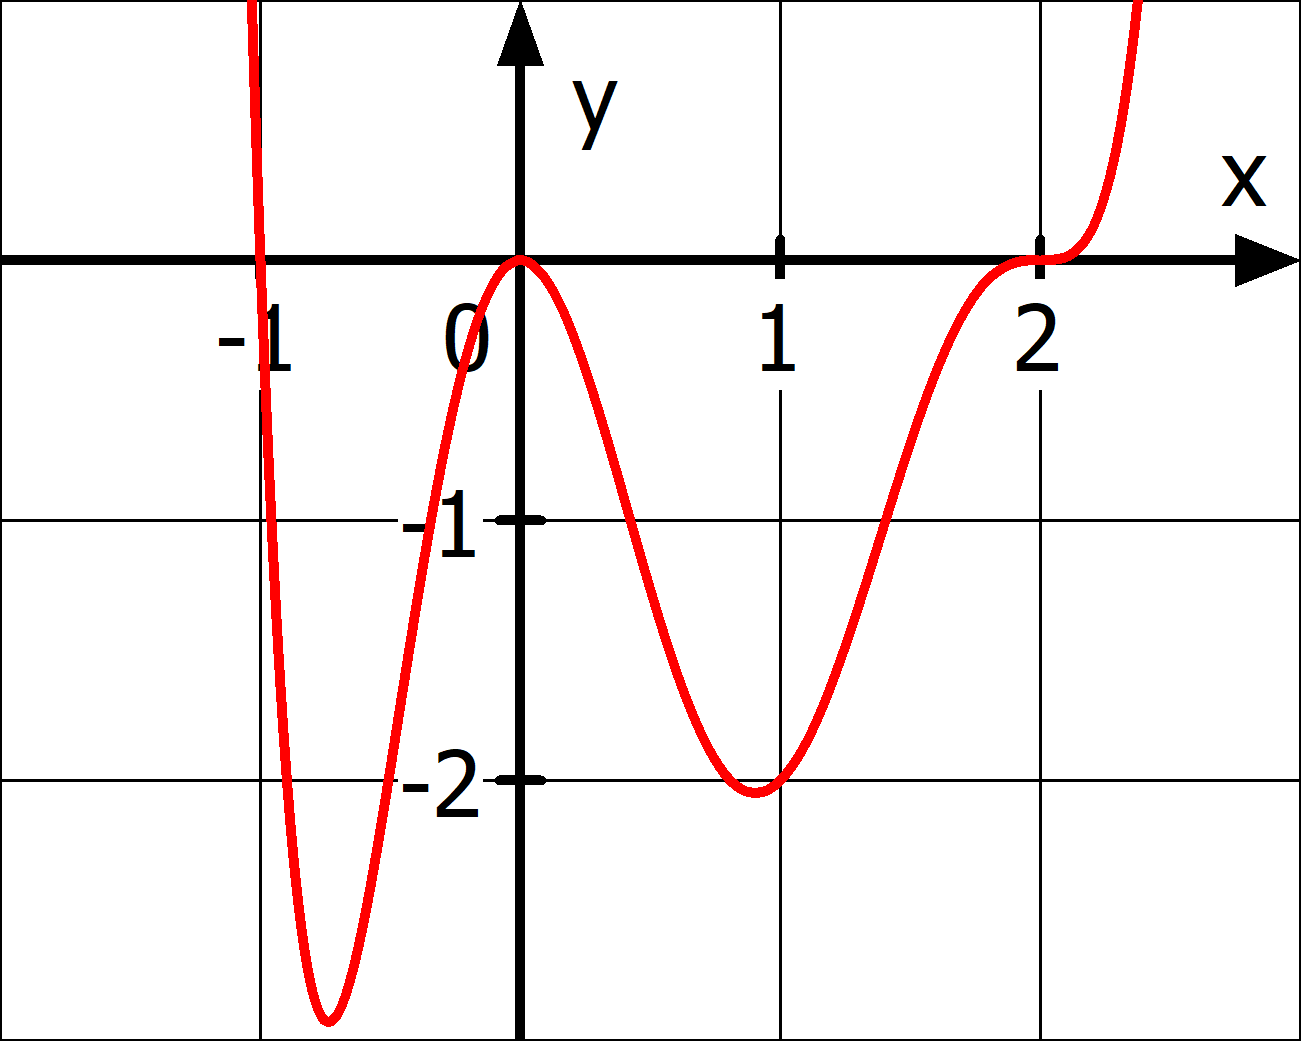
\includegraphics[width=\textwidth]{\quadFkt/pics/produkt1.png}
		\end{minipage}}%
		\adjustbox{valign=t, padding=0ex 0ex 3ex 0ex}{\begin{minipage}{\textwidth/\real{3}-2ex}\centering
			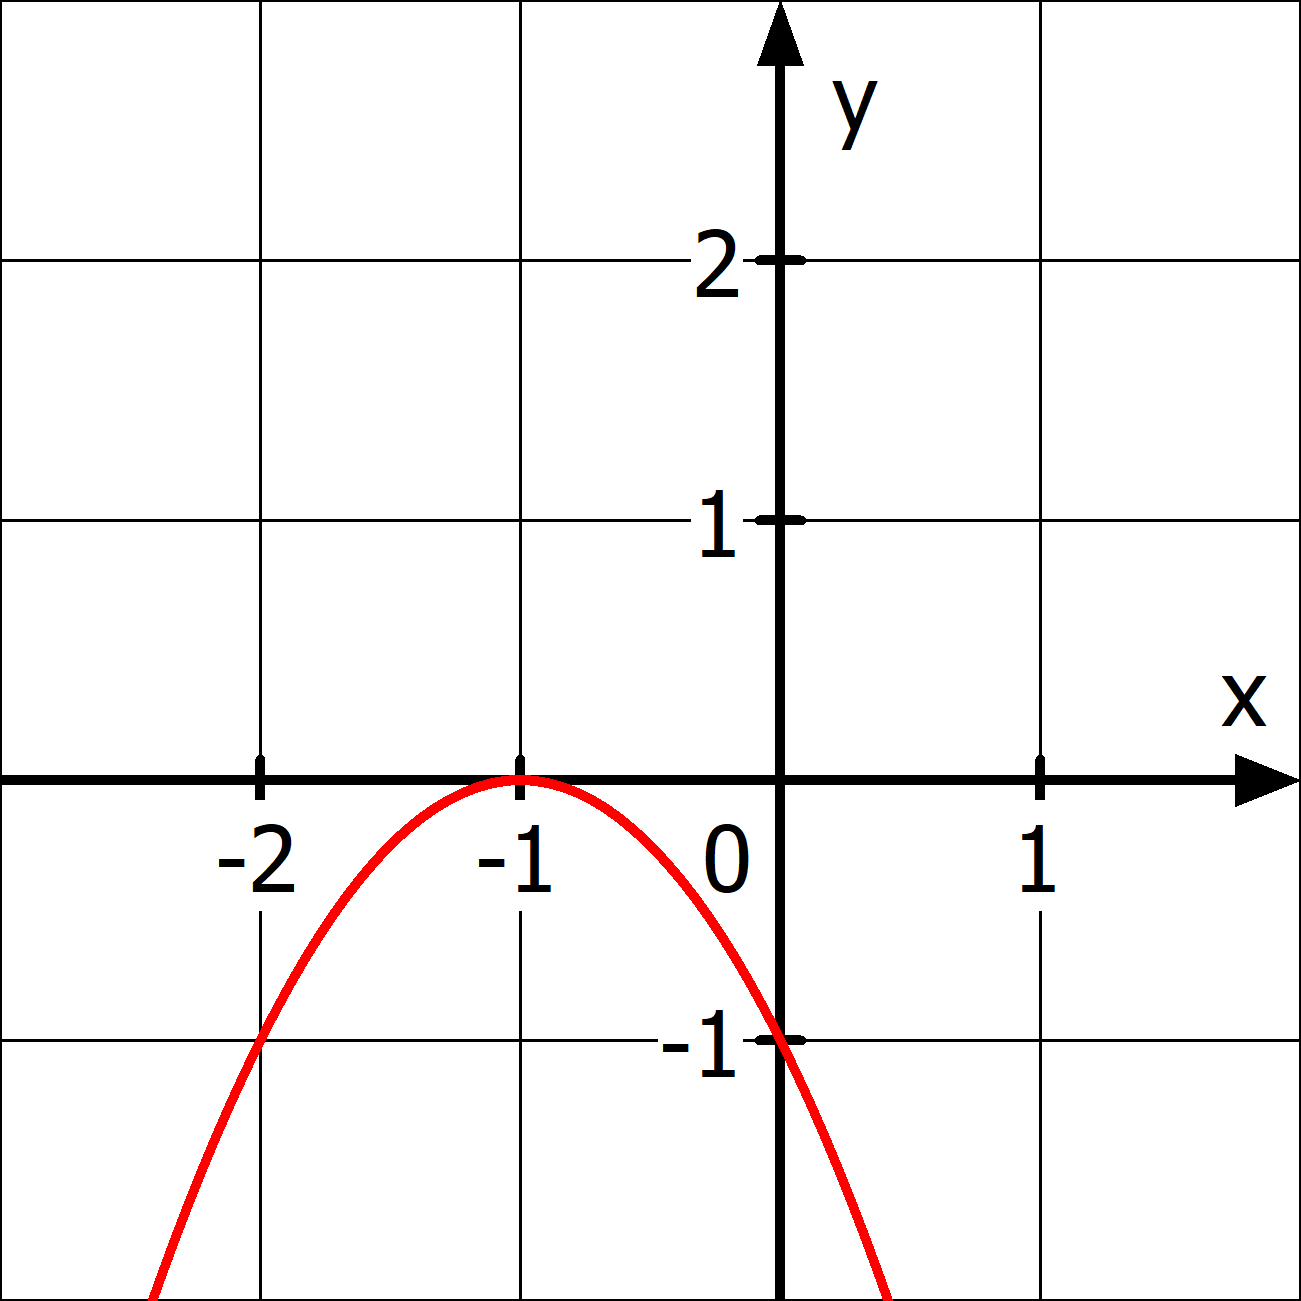
\includegraphics[width=\textwidth]{\quadFkt/pics/produkt2.png}
		\end{minipage}}%
		\adjustbox{valign=t}{\begin{minipage}{\textwidth/\real{3}-2ex}\centering
			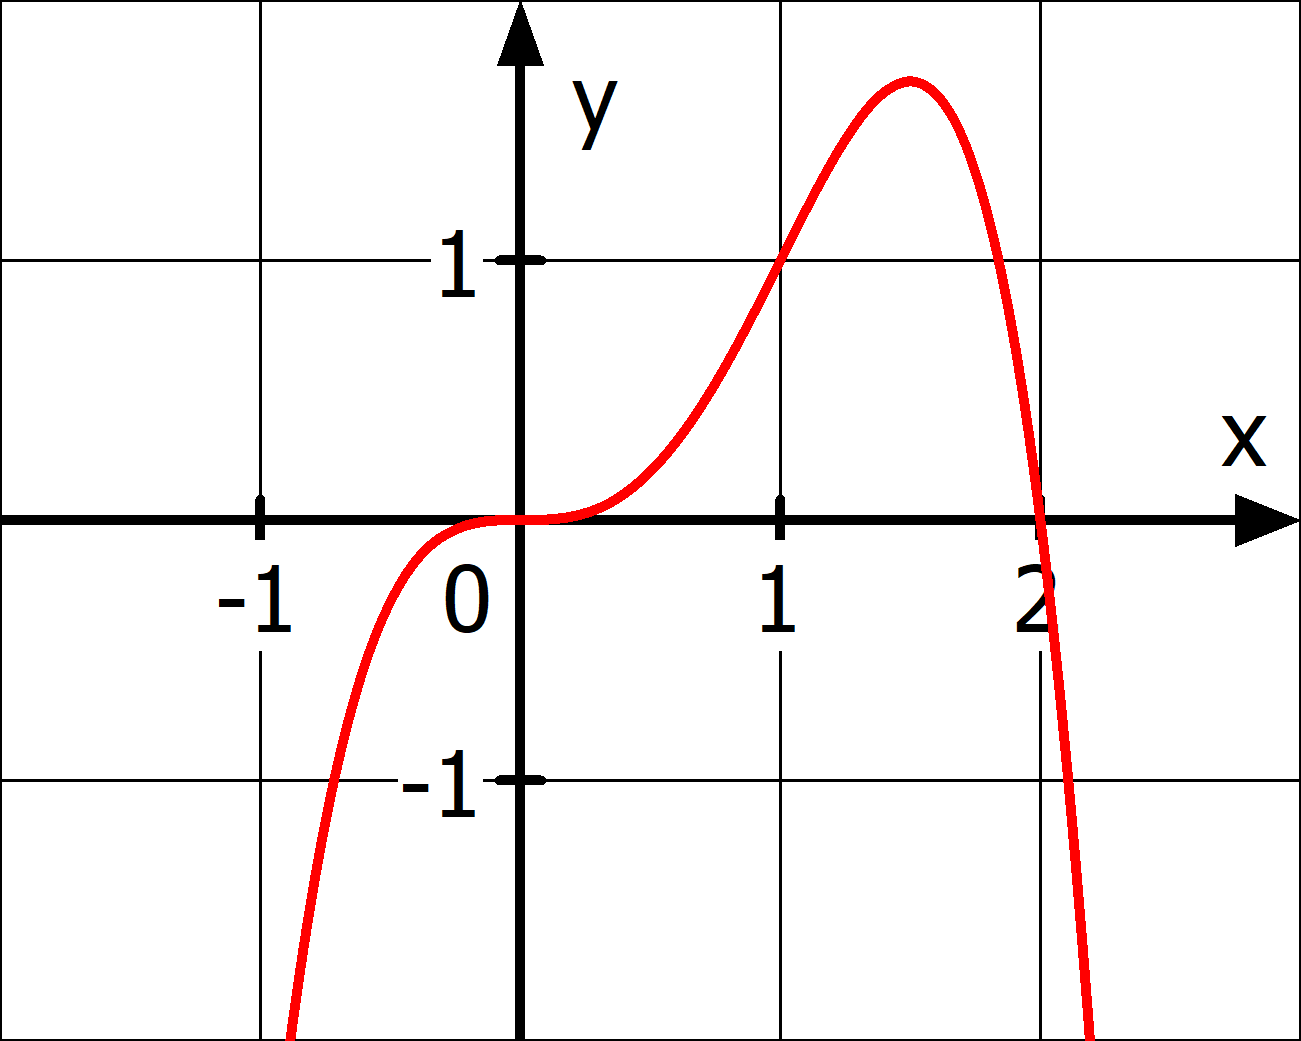
\includegraphics[width=\textwidth]{\quadFkt/pics/produkt3.png}
		\end{minipage}}%

		\bigskip

		\adjustbox{valign=t}{\begin{minipage}{\textwidth/\real{3}}\centering
			\[f_1(x)=\frac{3}{4}\left(x\textcolor{loes}{+2}\right)\left(x\textcolor{loes}{-1}\right)\]

			\textcolor{loes}{Nullstellen: \(x_1= -2,\quad x_2=1\)}
		\end{minipage}}%
		\adjustbox{valign=t}{\begin{minipage}{\textwidth/\real{3}}\centering
			\begin{align*}
			f_2(x)&=-\left(x\textcolor{loes}{+1}\right)\left(x\textcolor{loes}{+1}\right)\\
			&\textcolor{loes}{\;=-\left(x+1\right)^2}
			\end{align*}

			\textcolor{loes}{Nullstellen: \(x_{1/2}= -1\)}

			\textcolor{loes}{Doppelte Nullstelle}
		\end{minipage}}%
		\adjustbox{valign=t}{\begin{minipage}{\textwidth/\real{3}}\centering
			\[f_3(x)=x^2+1\]

			\textcolor{loes}{Keine Nullstellen, daher keine Produktform möglich.}
		\end{minipage}}%
\end{minipage}%
\vspace{1.8cm}
\newpage

%%%%%%%%%%%%%%%%%%%%%%%%%%%%%%%%%%%%%%%%%

\begin{Exercise}[title={Bestimme die Nullstellen}, label=produktformNullstellenA1]\\
	\begin{minipage}{\textwidth}
		\begin{minipage}{0.5\textwidth}
			\begin{enumerate}[label=\alph*)]
				\item \(f(x)=3\left(x+2\right)\left(x-4\right)\)
				\item \(f(x)=-2\left(x+8\right)\left(x+6\right)\)
				\item \(f(x)=5\left(x-2\right)x\)
				\item \(f(x)=-\frac{3}{4}\left(x+\frac{7}{5}\right)\left(x-\frac{4}{3}\right)\)
				\item \(f(x)=\sqrt{3}\left(x-10\right)^2\)
				\item \(f(x)=\left(x+\sqrt{2}\right)\left(x-3,8\right)\)
				\item \(f(x)=-\left(x-\frac{1}{2}\right)\left(x-\frac{3}{4}\right)\)
			\end{enumerate}
		\end{minipage}%
		\begin{minipage}{0.5\textwidth}
			\begin{enumerate}[label=\alph*)]
				\setcounter{enumi}{7}
				\item \(f(x)=10\left(x+\frac{8}{5}\right)\left(x-\frac{3}{5}\right)\)
				\item \(f(x)=-9x\left(x+9\right)\)
				\item \(f(x)=1,8\left(x-2,1\right)\left(x-5,9\right)\)
				\item \(f(x)=-8\left(x-\sqrt{5}\right)\left(x+\sqrt{11}\right)\)
				\item \(f(x)=-\frac{6}{5}\left(x-2\right)^2\)
				\item \(f(x)=\sqrt{3}\left(x-10\right)\left(x+8\right)\)
				\item \(f(x)=-2\left(x+17\right)\left(x+1\right)\)
			\end{enumerate}
		\end{minipage}%
	\end{minipage}%
\end{Exercise}

\begin{Exercise}[title={Bestimme die Nullstellen und skizziere das Schaubild}, label=produktformNullstellenA2]

	\begin{minipage}{\textwidth}
		\begin{minipage}{0.5\textwidth}
			\begin{enumerate}[label=\alph*)]
				\item \(f(x)=0,2\left(x+3\right)\left(x-2\right)\)
				\item \(g(x)=-0,5\left(x+5\right)\left(x+2\right)\)
			\end{enumerate}
		\end{minipage}%
		\begin{minipage}{0.5\textwidth}
			\begin{enumerate}[label=\alph*)]
				\setcounter{enumi}{2}
				\item \(h(x)=\left(x+1\right)^2\)
				\item \(i(x)=-\frac{1}{2}x\left(x-\frac{3}{2}\right)\)
			\end{enumerate}
		\end{minipage}%
	\end{minipage}%
\end{Exercise}

\newpage
%%%%%%%%%%%%%%%%%%%%%%%%%%%%%%%%%%%%%%%%%
\begin{Answer}[ref=produktformNullstellenA1]

	\begin{minipage}{\textwidth}
		\begin{minipage}{0.5\textwidth}
			\begin{enumerate}[label=\alph*)]
				\item \(x_1=-2,\quad x_2=4\)
				\item \(x_1=-8,\quad x_2=-6\)
				\item \(x_1=2,\quad x_2=0\)
				\item \(x_1=-\frac{7}{5},\quad x_2=\frac{4}{3}\)
				\item \(x_{1/2}=10\)
				\item \(x_1=-\sqrt{2},\quad x_2=3,8\)
				\item \(x_1=\frac{1}{2},\quad x_2=\frac{3}{4}\)
			\end{enumerate}
		\end{minipage}%
		\begin{minipage}{0.5\textwidth}
			\begin{enumerate}[label=\alph*)]
				\setcounter{enumi}{7}
				\item \(x_1=-\frac{8}{5},\quad x_2=\frac{3}{5}\)
				\item \(x_1=0,\quad x_2=-9\)
				\item \(x_1=2,1,\quad x_2=5,9\)
				\item \(x_1=\sqrt{5},\quad x_2=-\sqrt{11}\)
				\item \(x_{1/2}=2\)
				\item \(x_1=10,\quad x_2=-8\)
				\item \(x_1=-17,\quad x_2=-1\)
			\end{enumerate}
		\end{minipage}%
	\end{minipage}%
\end{Answer}
\begin{Answer}[ref=produktformNullstellenA2]

	\begin{minipage}{\textwidth}
		\begin{minipage}{0.5\textwidth}
			\begin{enumerate}[label=\alph*)]
				\item \(\textcolor{red}{x_1=-3,\quad x_2=2}\)
				\item \(\textcolor{blue}{x_1=-5,\quad x_2=-2}\)
			\end{enumerate}
		\end{minipage}%
		\begin{minipage}{0.5\textwidth}
			\begin{enumerate}[label=\alph*)]
				\setcounter{enumi}{2}
				\item \(\textcolor{ForestGreen}{x_{1/2}=-1}\)
				\item \(\textcolor{YellowOrange}{x_1=0,\quad x_2=-\frac{3}{2}}\)
			\end{enumerate}
		\end{minipage}%
	\end{minipage}%

	\bigskip

	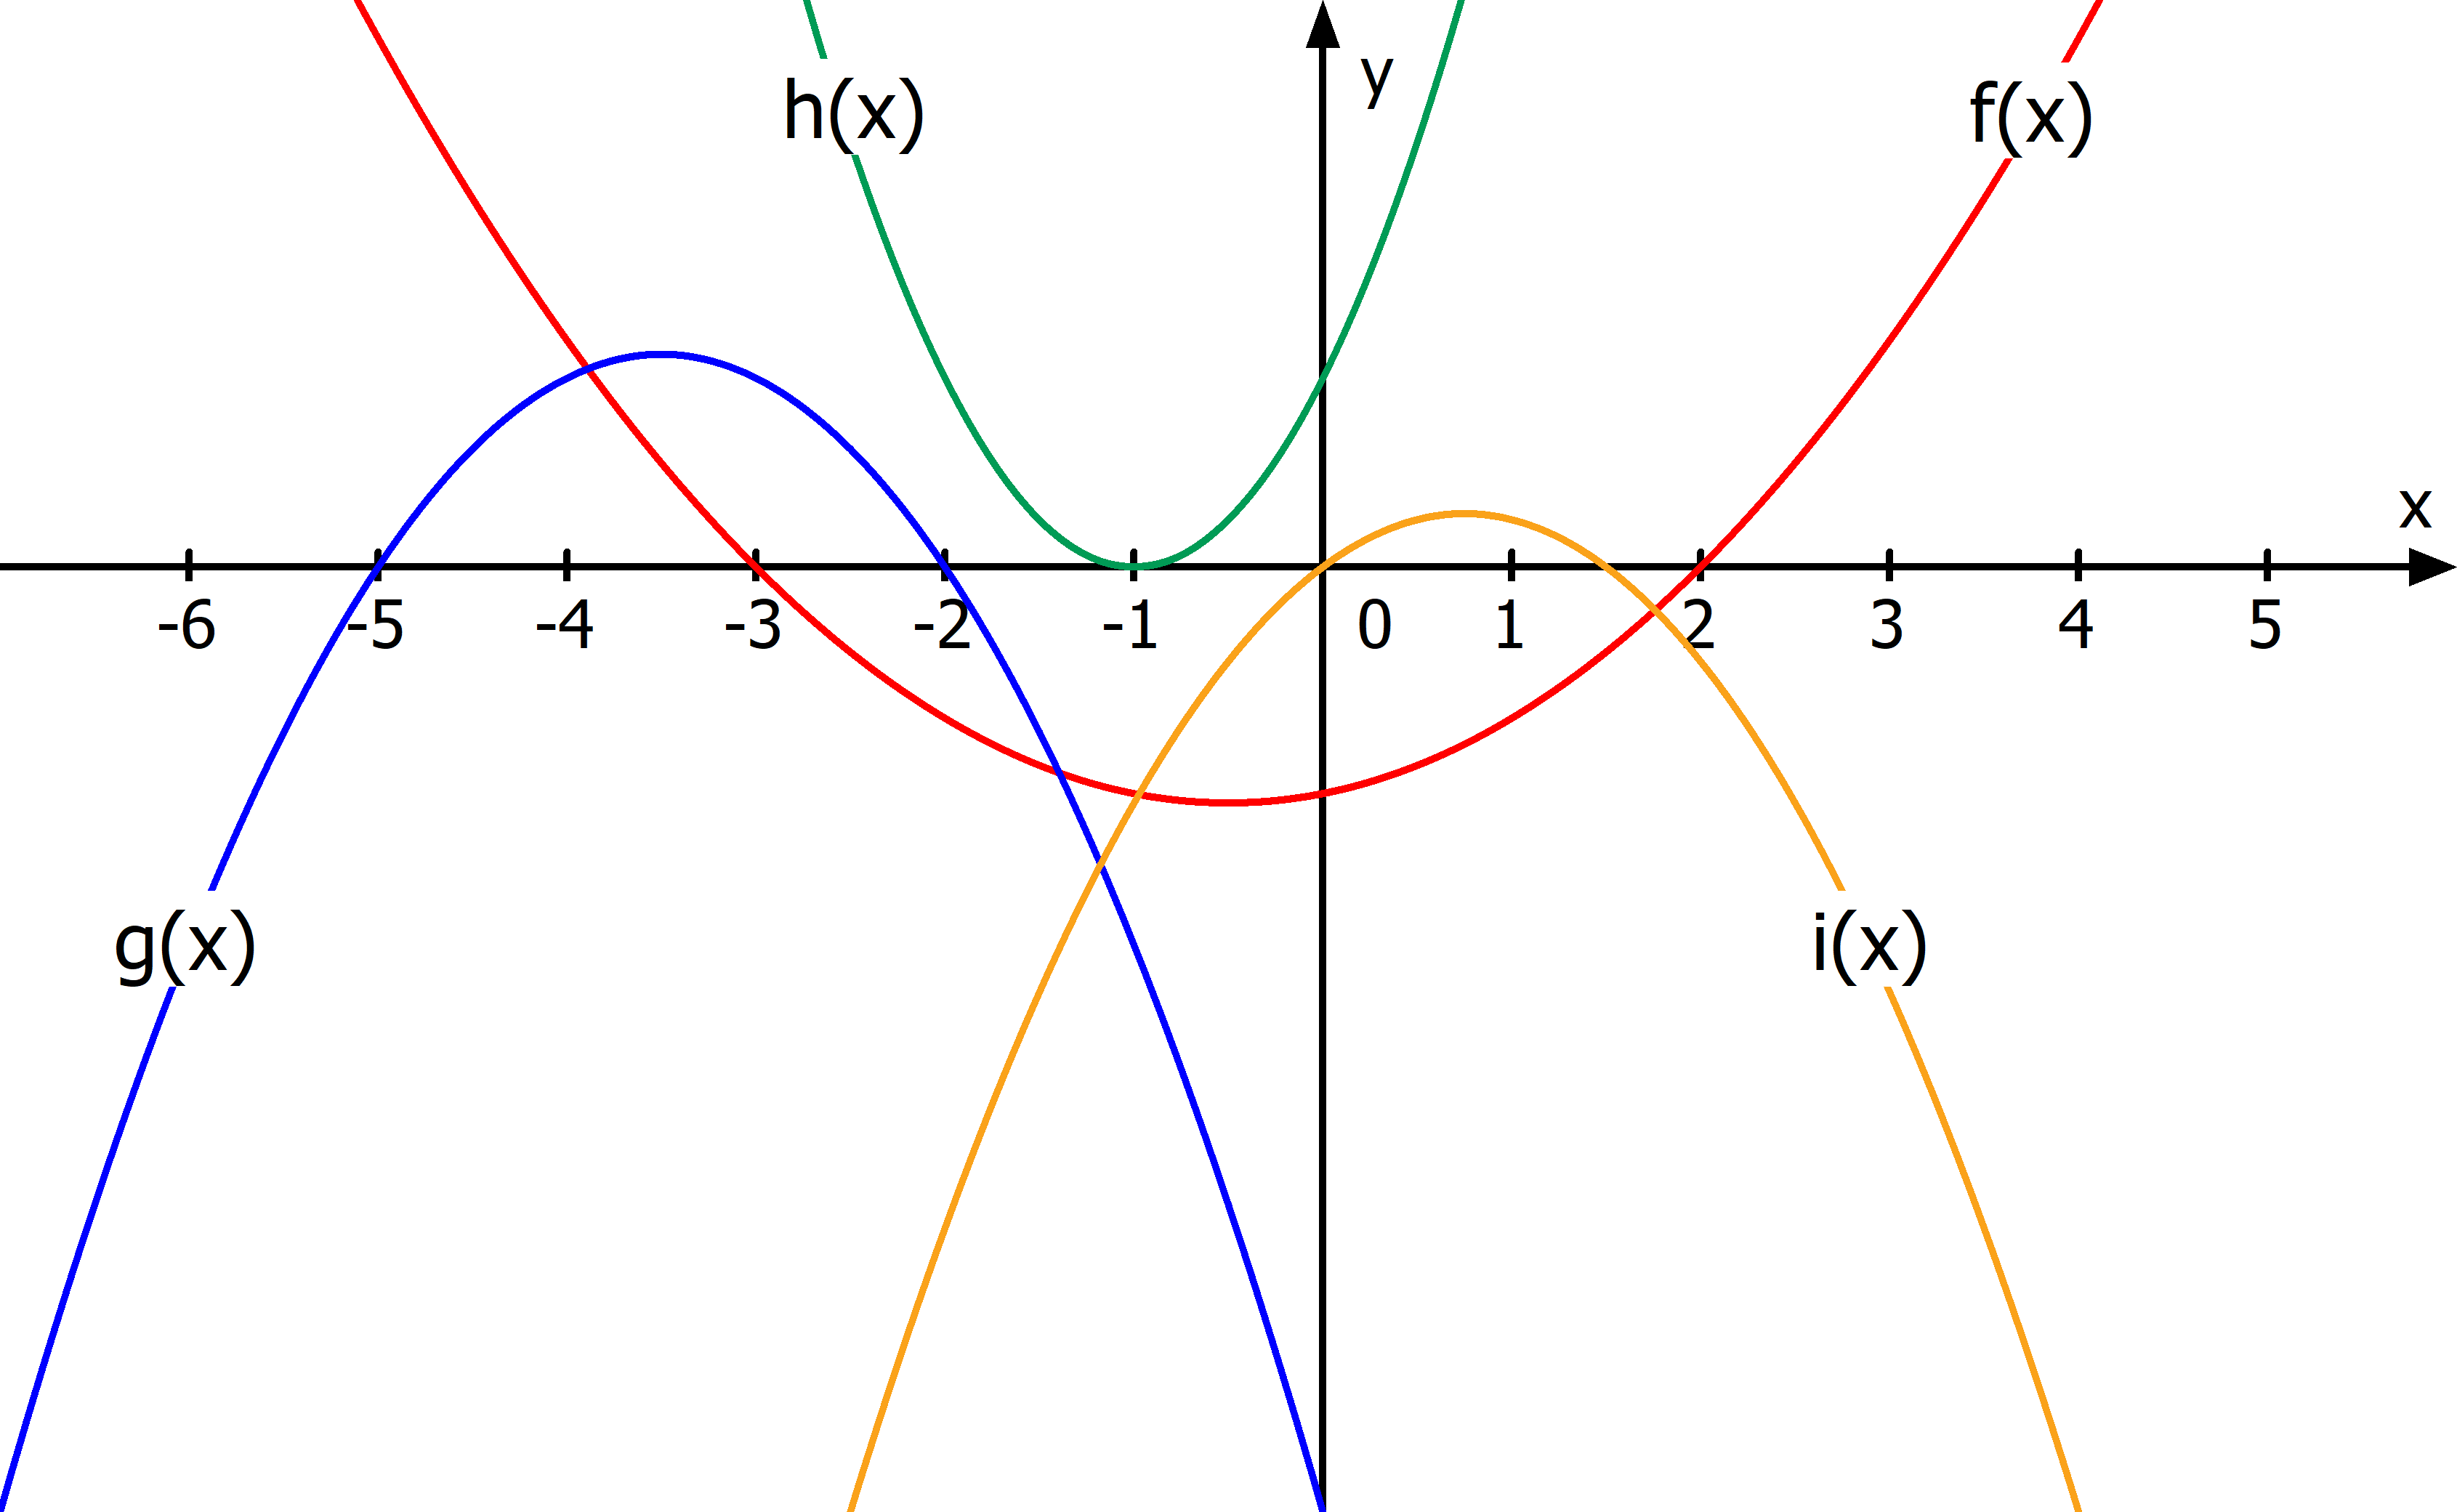
\includegraphics[width=\textwidth]{\quadFkt/pics/produktA2.png}
\end{Answer}